\documentclass[t]{beamer}
\usepackage[utf8]{inputenc}  % to be able to type unicode text directly
%\usepackage[french]{babel}   % french typographical conventions
\usepackage{inconsolata}     % for a nicer (e.g. non-courier) tt family font
%\usepackage{amsthm,amsmath}  % fancier mathematics
\usepackage{array} % to fine-tune tabular spacing
\usepackage{bbm} % for blackboard 1

\usepackage{graphicx}        % to include images
%\usepackage{animate}         % to include animated images
\usepackage{soul}            % for colored strikethrough
%\usepackage{bbding}          % for Checkmark and XSolidBrush
\usepackage{hyperref,url}

\colorlet{darkgreen}{black!50!green}  % used for page numbers
\definecolor{term}{rgb}{.9,.9,.9}     % used for code insets

\setlength{\parindent}{0em}
\setlength{\parskip}{1em}


% coco's macros
\def\R{\mathbf{R}}
\def\F{\mathcal{F}}
\def\x{\mathbf{x}}
\def\y{\mathbf{y}}
\def\u{\mathbf{u}}
\def\Z{\mathbf{Z}}
\def\d{\mathrm{d}}
\DeclareMathOperator*{\argmin}{arg\,min}
\DeclareMathOperator*{\argmax}{arg\,max}
\newcommand{\reference}[1] {{\scriptsize \color{gray}  #1 }}
\newcommand{\referencep}[1] {{\tiny \color{gray}  #1 }}
\newcommand{\unit}[1] {{\tiny \color{gray}  #1 }}

% disable spacing around verbatim
\usepackage{etoolbox}
\makeatletter\preto{\@verbatim}{\topsep=0pt \partopsep=0pt }\makeatother

% disable headings, set slide numbers in green
\mode<all>\setbeamertemplate{navigation symbols}{}
\defbeamertemplate*{footline}{pagecount}{\leavevmode\hfill\color{darkgreen}
   \insertframenumber{} / \inserttotalframenumber\hspace*{2ex}\vskip0pt}

%% select red color for strikethrough
\makeatletter
\newcommand\SoulColor{%
  \let\set@color\beamerorig@set@color
  \let\reset@color\beamerorig@reset@color}
\makeatother
\newcommand<>{\St}[1]{\only#2{\SoulColor\st{#1}}}
\setstcolor{red}

% make everything monospace
\renewcommand*\familydefault{\ttdefault}

\begin{document}

\begin{frame}[plain,fragile]
\LARGE
\begin{verbatim}






        S5P L1 CH4 POC





\end{verbatim}
\end{frame}

% \begin{frame}
% 	ALISO CANYON 2015 (apparently, SWIR)
% 
% 	\includegraphics[width=\linewidth]{f/aliso.jpg}
% \end{frame}

\begin{frame}
SUMMARY\\
=======


1. Overview of Sentinel 5P raw data (Level 1b)

2. Extraction of a methane signal from L1b data\\
\pause
(Note: a {\bf signal}, not a {\bf measure})
\pause
\begin{tabular}{ll}
	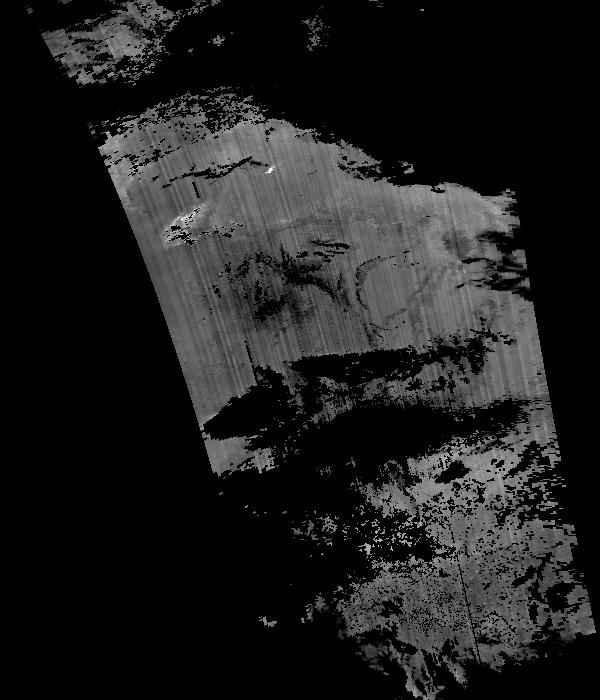
\includegraphics[height=.6\textheight]{f/ccplume20.png} &
	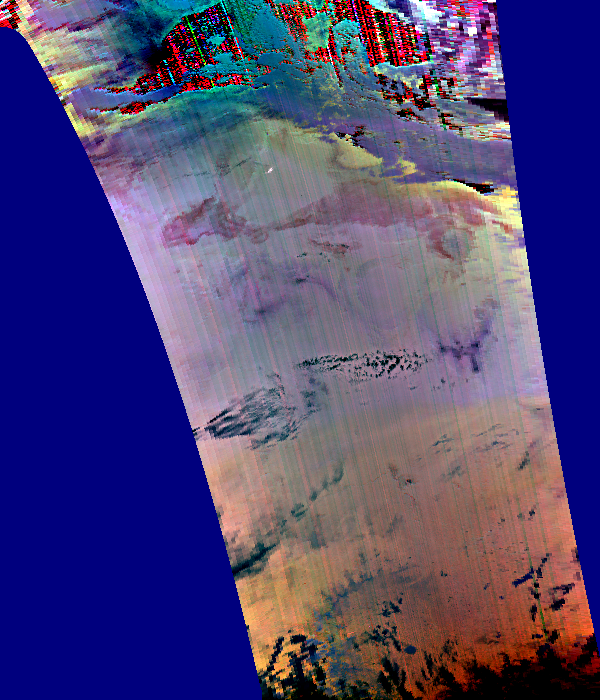
\includegraphics[height=.6\textheight]{f/niceshot.png}
\end{tabular}
\end{frame}

\begin{frame}
	\tiny RGB composite from full S5P spectrum
	\hspace{3em} \only<2>{false color rendering}\\
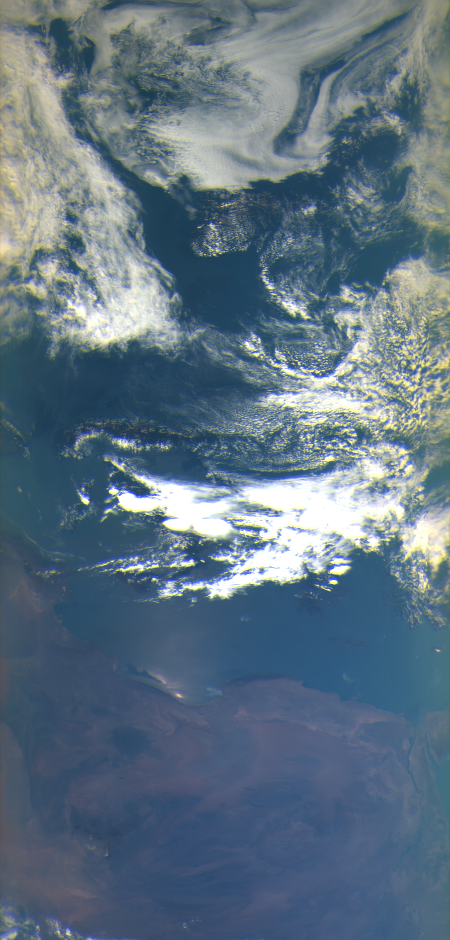
\includegraphics[height=\textheight]{f/s5p_visible.png}
\pause
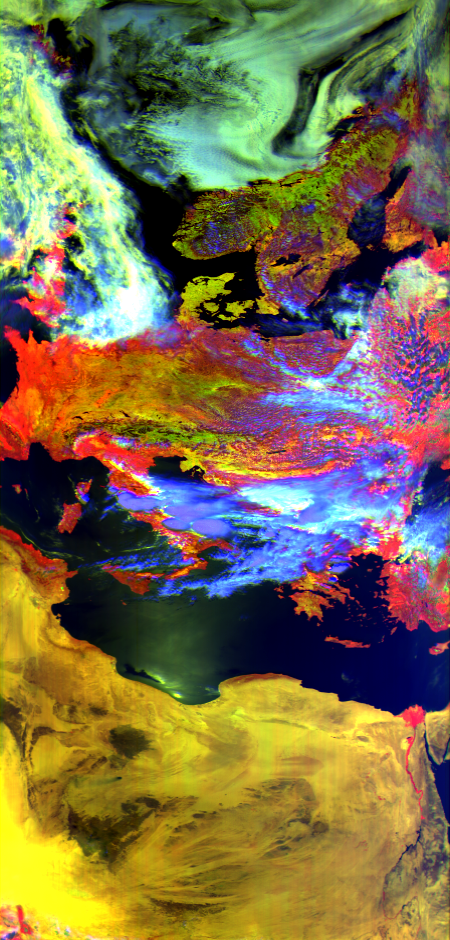
\includegraphics[height=\textheight]{f/s5p_falsecolor3.png}
\end{frame}



\begin{frame}[fragile]
\begin{verbatim}
OVERVIEW OF SENTINEL-5P LEVEL-1 DATA
====================================

The TROPOMI instrument provides 8 multi-spectral "bands":

band meter  width  height  freqs  km/pix        nm range
1    UV     77     3246    497    20.0 x 3.5    270--300
2    UV     448    3246    497     3.5 x 3.5    300--330
3    UVIS   450    3246    497     3.5 x 3.5    312--405
4    UVIS   450    3246    497     3.5 x 3.5    405--500
5    NIR    448    3246    497     3.5 x 3.5    675--725
6    NIR    448    3246    497     3.5 x 3.5    725--775
7    SWIR   215    3246    480     7.0 x 3.5   2305-2345
8    SWIR   215    3246    480     7.0 x 3.5   2345-2385

There are about 15 such products per day,
for a daily global coverage (about 20GB/product, 300GB/day).
\end{verbatim}
%\small
%\begin{verbatim}
%OVERVIEW OF SENTINEL-5P LEVEL-1 DATA
%====================================
%
%The TROPOMI instrument provides 8 multi-spectral "bands":
%
%band meter  width  height  depth  size    km/pix (WxH)  nm range
%1    UV     77     3246    497    0.5GB   20.0 x 3.5    270--300
%2    UV     448    3246    497    2.8GB    3.5 x 3.5    300--320
%3    UVIS   450    3246    497    2.8GB    3.5 x 3.5    320--405
%4    UVIS   450    3246    497    2.6GB    3.5 x 3.5    405--500
%5    NIR    448    3246    497    2.6GB    3.5 x 3.5    675--725
%6    NIR    448    3246    497    2.7GB    3.5 x 3.5    725--775
%7    SWIR   215    3246    480    1.5GB    7.0 x 3.5   2305-2345
%8    SWIR   215    3246    480    1.5GB    7.0 x 3.5   2345-2385
%            450    3246    3930  17.0GB                        .
%
%There are about 15 such products per day,
%for a daily global coverage.
%\end{verbatim}
\end{frame}

%SCRIPT cat <<END | gnuplot > f/whole2_c19.png
%SCRIPT set term pngcairo crop size 900,600
%SCRIPT plot "dat/curv19_all" title "Constantine, 2019" pt 7 ps 0.5
%SCRIPT END

\begin{frame}
A SINGLE S5P PIXEL (3942 SPECTRAL SAMPLES)\\
==========================================

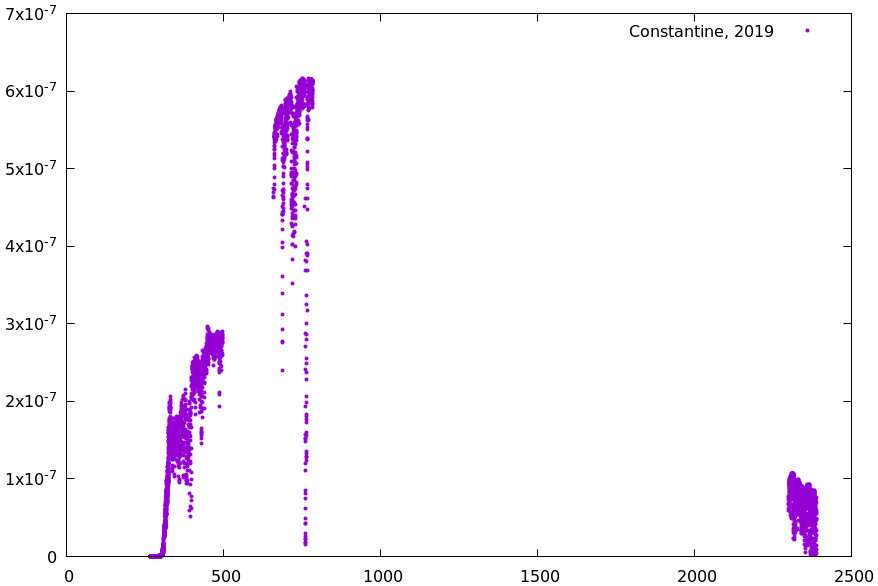
\includegraphics[width=\linewidth]{f/whole2_c19.png}
\end{frame}

%SCRIPT cat <<END | gnuplot > f/whole_c19.png
%SCRIPT set term pngcairo crop size 900,200
%SCRIPT plot "dat/curv19_all" title "Constantine, 2019" pt 7 ps 0.5
%SCRIPT END
%SCRIPT cat <<END | gnuplot > f/whole_c20.png
%SCRIPT set term pngcairo crop size 900,200
%SCRIPT plot "dat/curv20_all" title "Constantine, 2020" pt 7 ps 0.5
%SCRIPT END
%SCRIPT cat <<END | gnuplot > f/whole_k19.png
%SCRIPT set term pngcairo crop size 900,200
%SCRIPT plot "dat/kurv19_all" title "Ouargla, 2019 (no plume)" pt 7 ps 0.5
%SCRIPT END
%SCRIPT cat <<END | gnuplot > f/whole_k20.png
%SCRIPT set term pngcairo crop size 900,200
%SCRIPT plot "dat/kurv20_all" title "Ouargla, 2020 (plume)" pt 7 ps 0.5
%SCRIPT END

%\begin{frame}
%	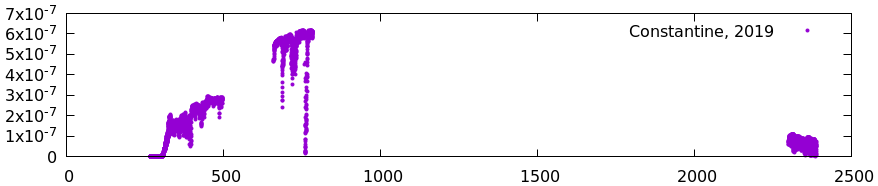
\includegraphics[width=\linewidth]{f/whole_c19.png}
%	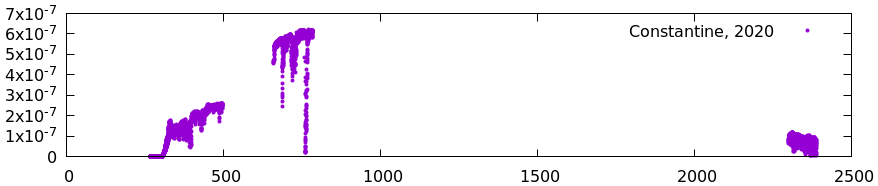
\includegraphics[width=\linewidth]{f/whole_c20.png}
%	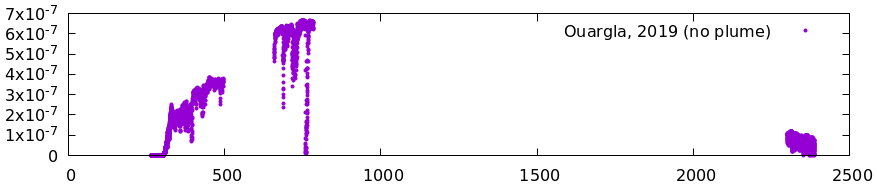
\includegraphics[width=\linewidth]{f/whole_k19.png}
%	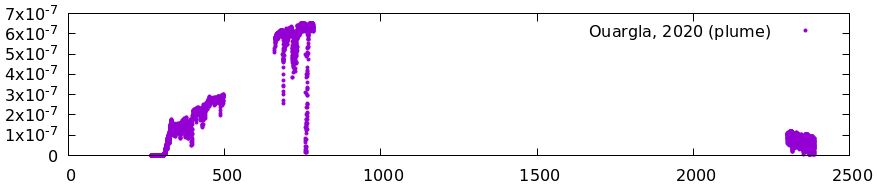
\includegraphics[width=\linewidth]{f/whole_k20.png}
%\end{frame}



\begin{frame}[fragile]
\begin{verbatim}
OTHER PRODUCTS (TO IGNORE)
==========================

We have just described the nominal L1 "RADIANCE" product,
but there are more:

The IRRADIANCE measures the daily spectrum of the sun.
It is a tiny dataset that concerns mostly the UV spectrum,
where the irradiance varies in a meaningful way.

The CALIBRATION is a full-resolution full-spectrum dataset
of about 20GB, measuring the biases of each pixel.
It concerns mostly the IR spectrum, where the sensor is
very delicate and subject to daily degradation.

The ENGINEERING dataset is acquired once per orbit.  It is
a small dataset of orbit calibration and instrument monitoring.
\end{verbatim}
\end{frame}


\begin{frame}
	\vspace*{-0.5em}
	\hspace*{-3.1em}
	\tiny
	\renewcommand{\tabcolsep}{0.2pt}
	\begin{tabular}{cccccccc}
		1 UV & 2 UV & 3 UVIS & 4 UVIS & 5 NIR & 6 NIR & 7 SWIR & 8 SWIR \\
		
\includegraphics[height=\textheight]{f/s5p_b1_avg.png} &
		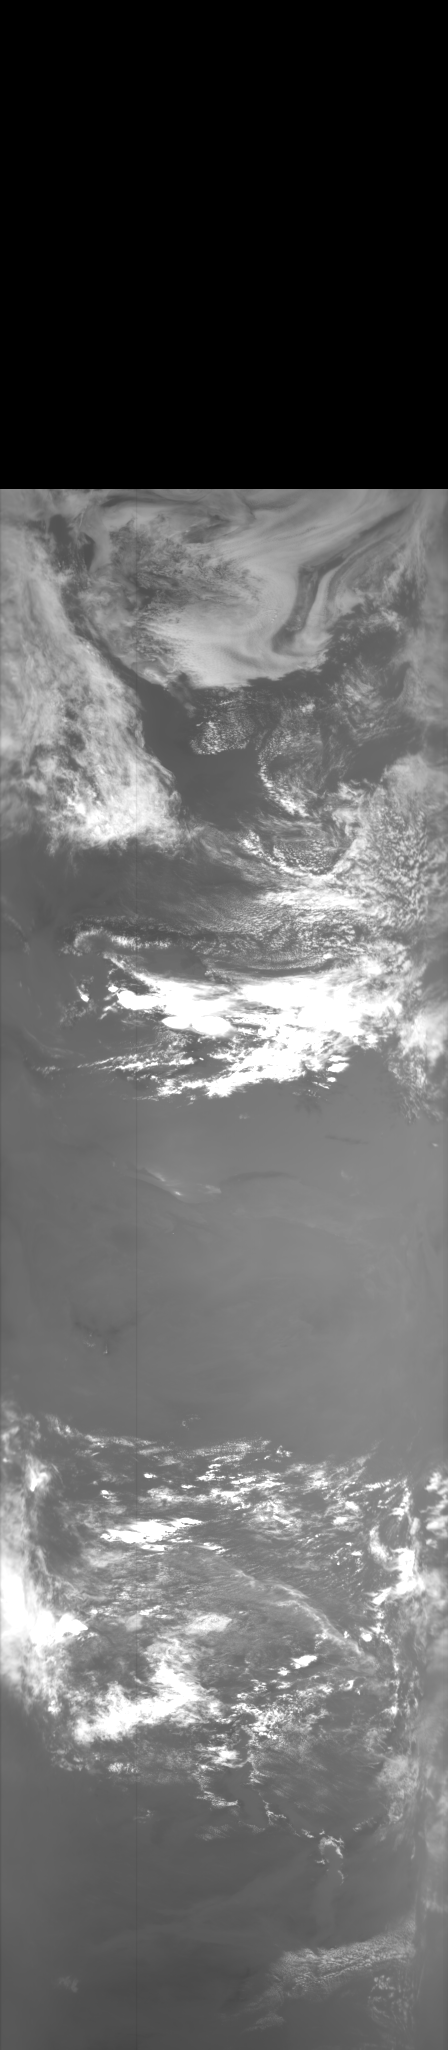
\includegraphics[height=\textheight]{f/s5p_b2_avg.png} &
		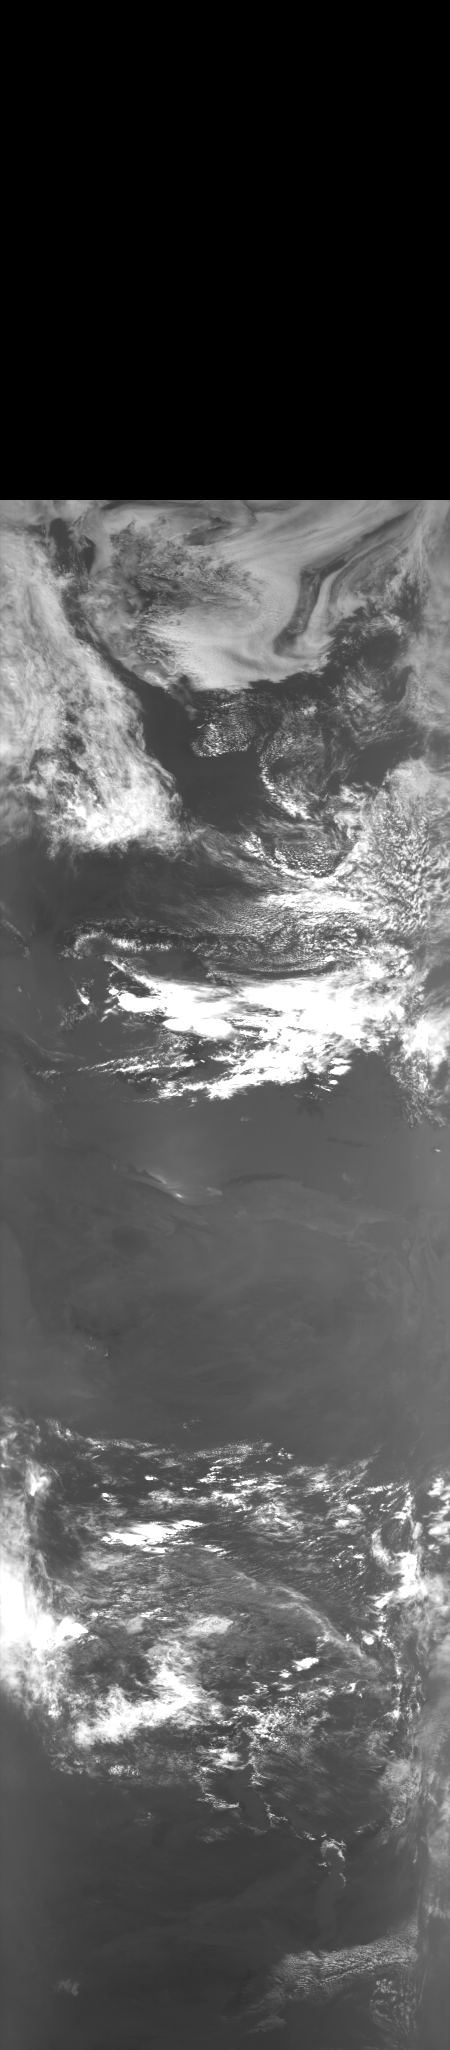
\includegraphics[height=\textheight]{f/s5p_b3_avg.png} &
		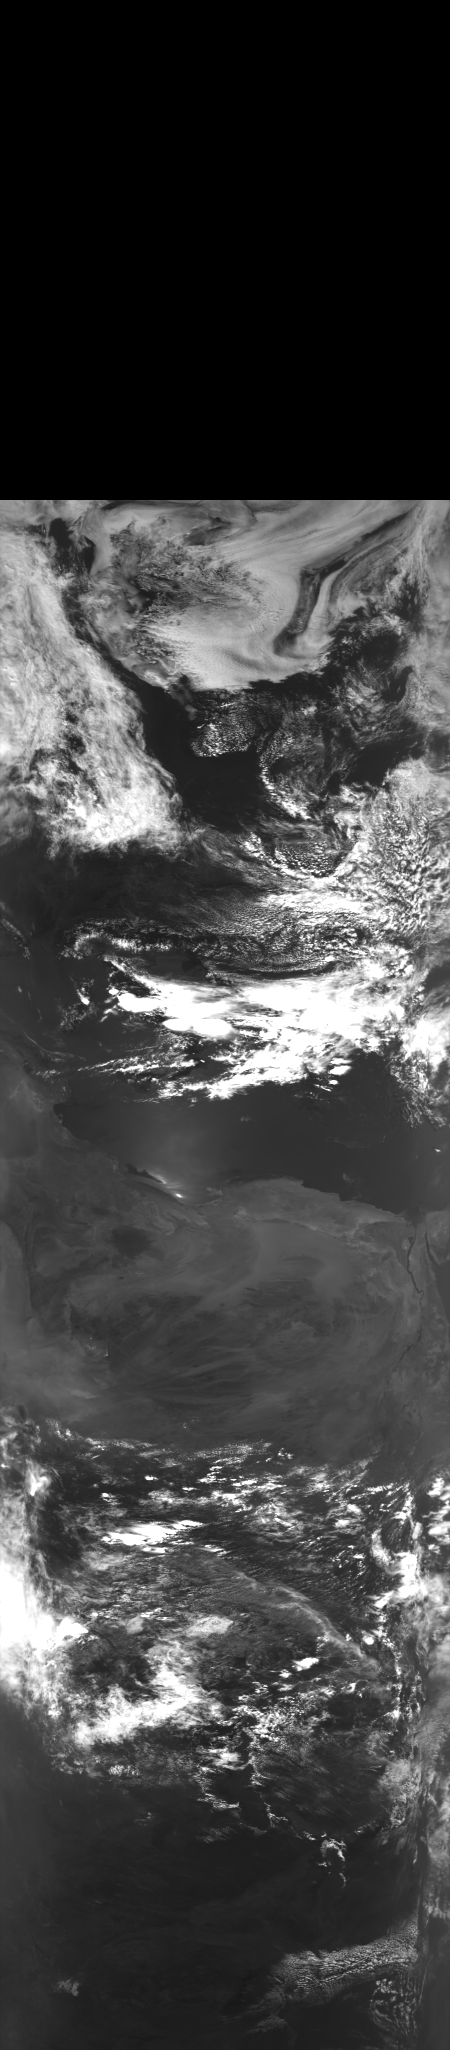
\includegraphics[height=\textheight]{f/s5p_b4_avg.png} &
		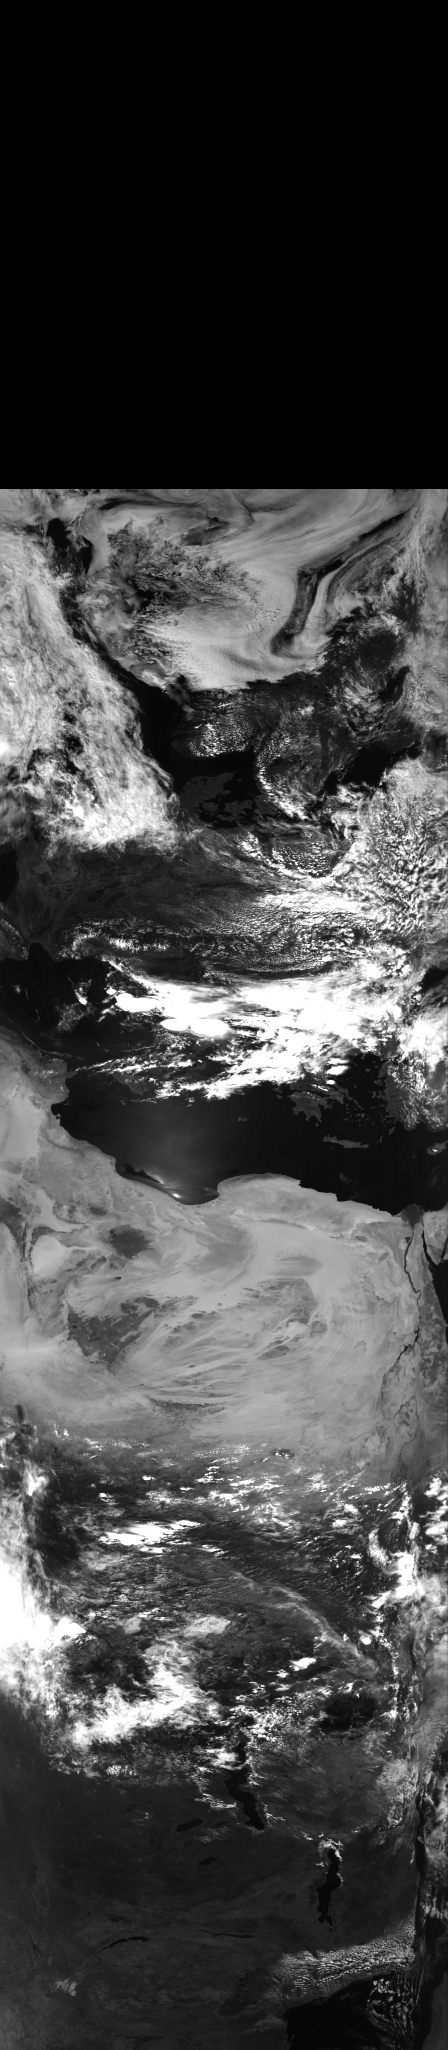
\includegraphics[height=\textheight]{f/s5p_b5_avg.png} &
		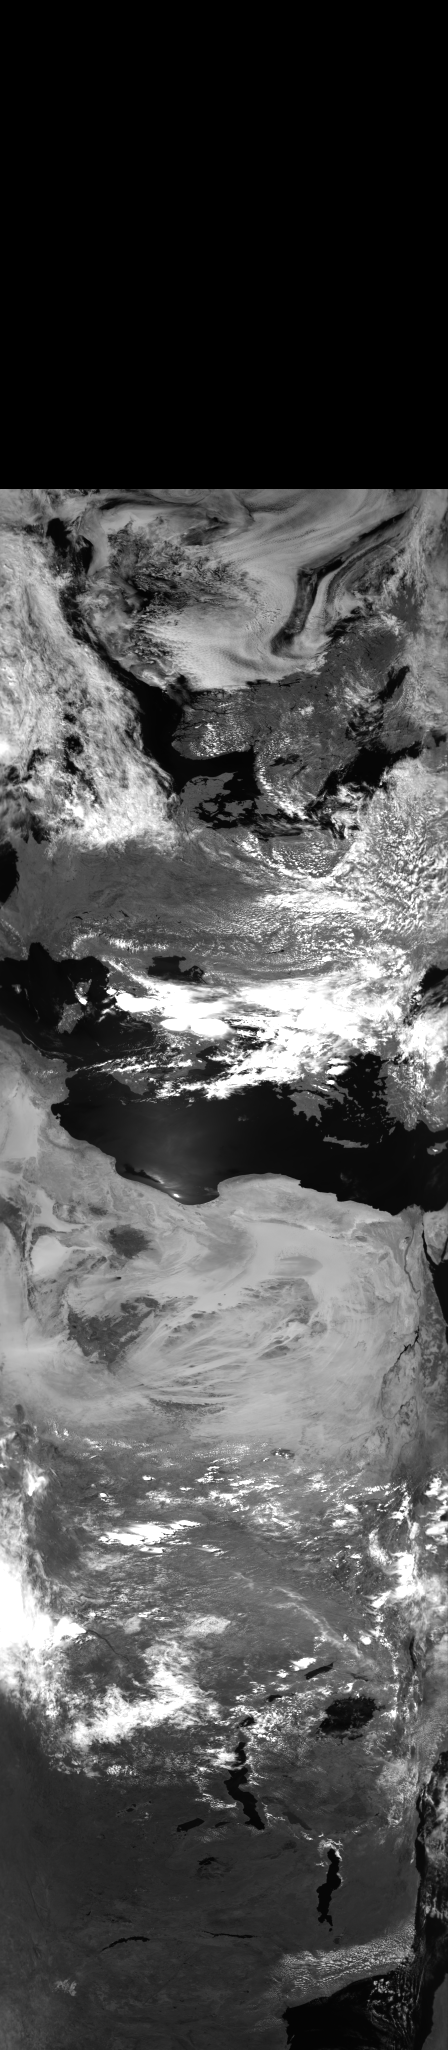
\includegraphics[height=\textheight]{f/s5p_b6_avg.png} &
		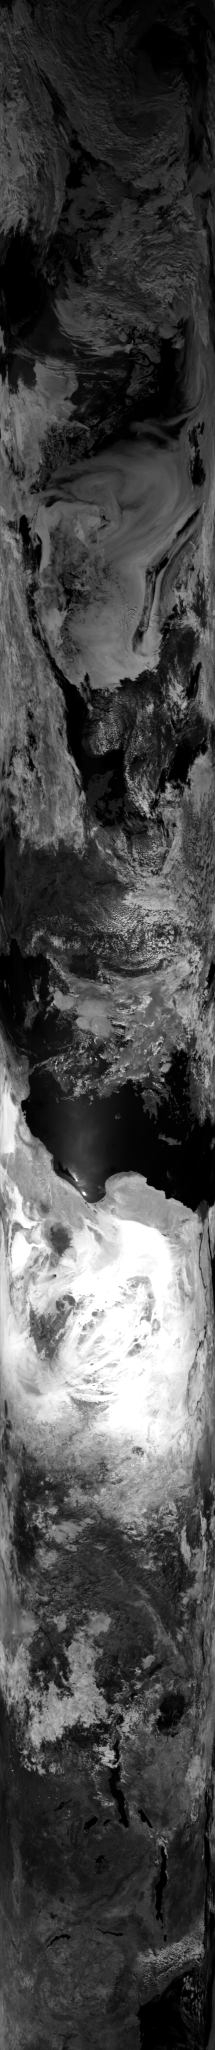
\includegraphics[height=\textheight]{f/s5p_b7_avg.png} &
		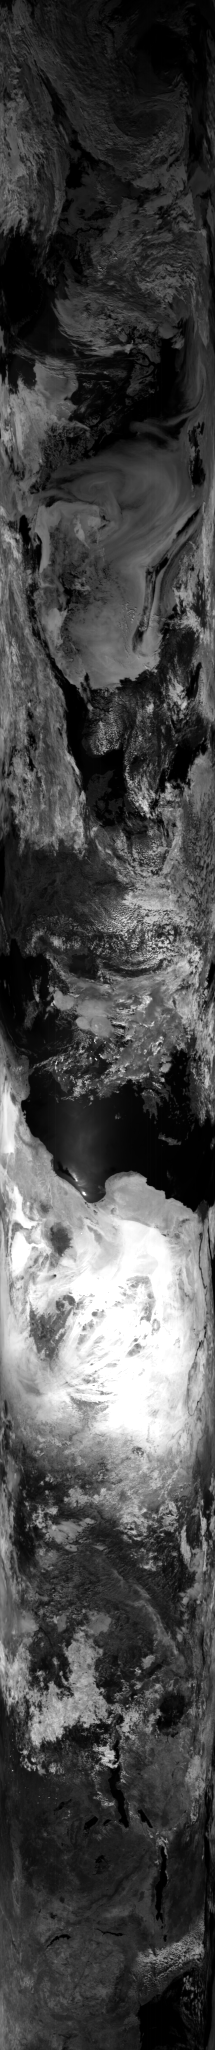
\includegraphics[height=\textheight]{f/s5p_b8_avg.png}
	\end{tabular}
\end{frame}

%\begin{frame}
%	\vspace*{-0.5em}
%	\hspace*{-3.1em}
%	\tiny
%	\renewcommand{\tabcolsep}{0.2pt}
%	\begin{tabular}{cccccccc}
%		1 UV & 2 UV & 3 UVIS & 4 UVIS & 5 NIR & 6 NIR & 7 SWIR & 8 SWIR \\
%		
\includegraphics[height=\textheight]{f/s5p_b1_std.png} &
%		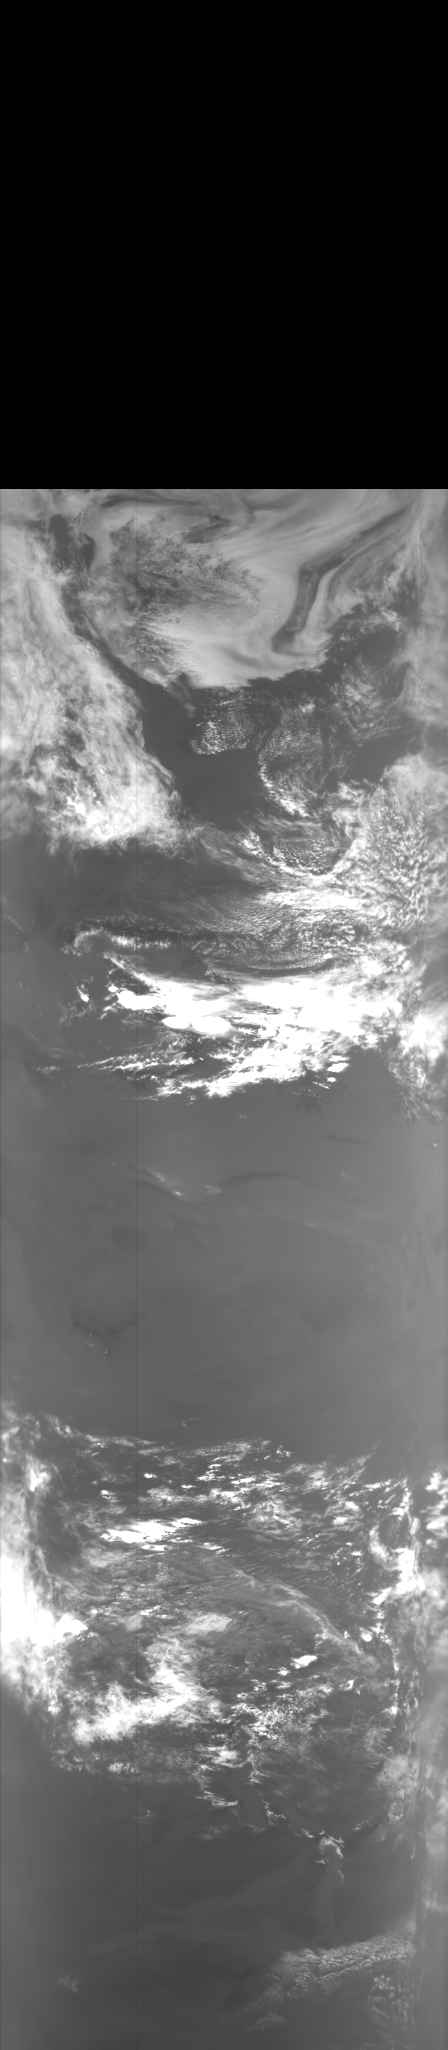
\includegraphics[height=\textheight]{f/s5p_b2_std.png} &
%		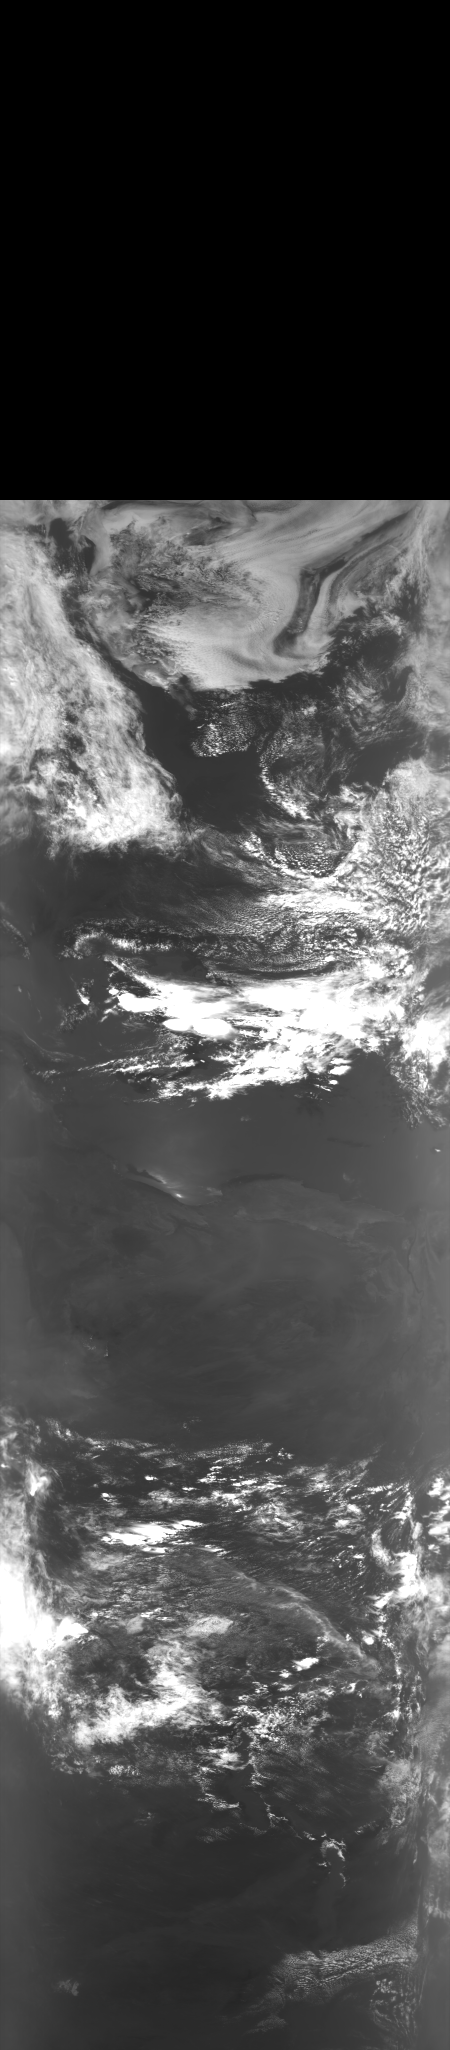
\includegraphics[height=\textheight]{f/s5p_b3_std.png} &
%		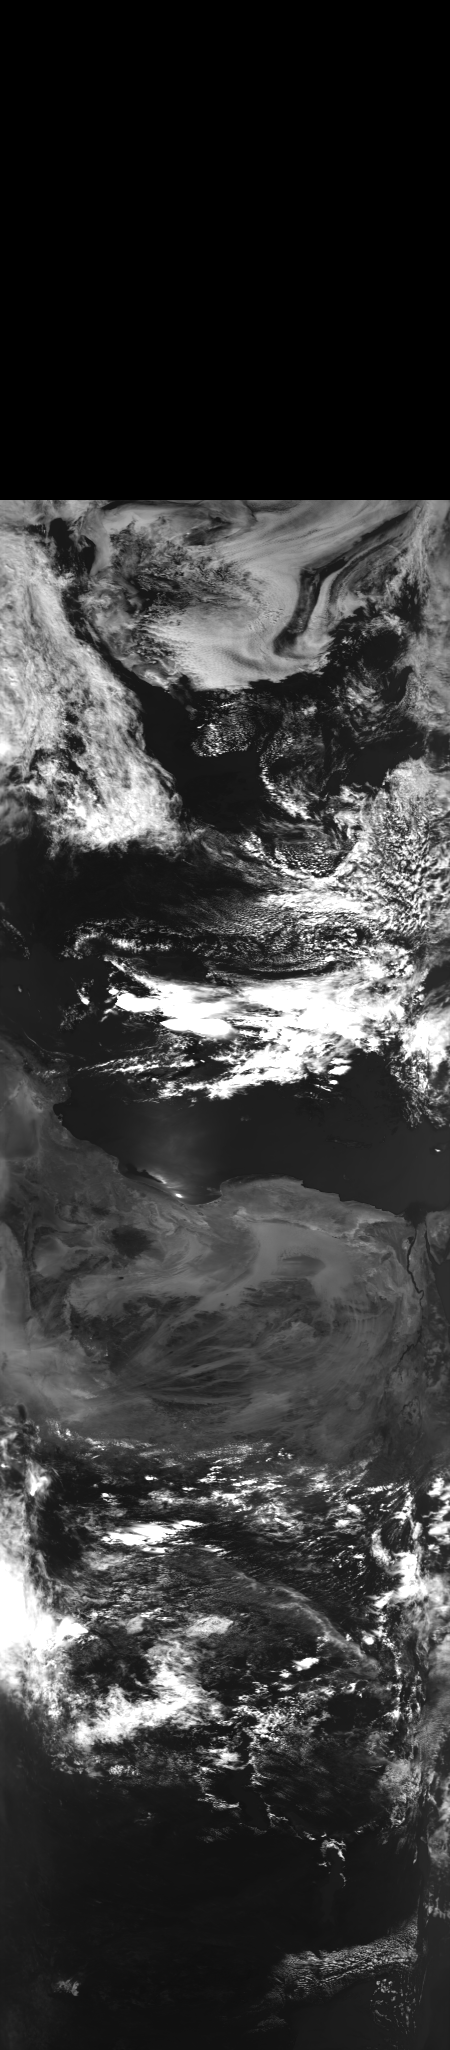
\includegraphics[height=\textheight]{f/s5p_b4_std.png} &
%		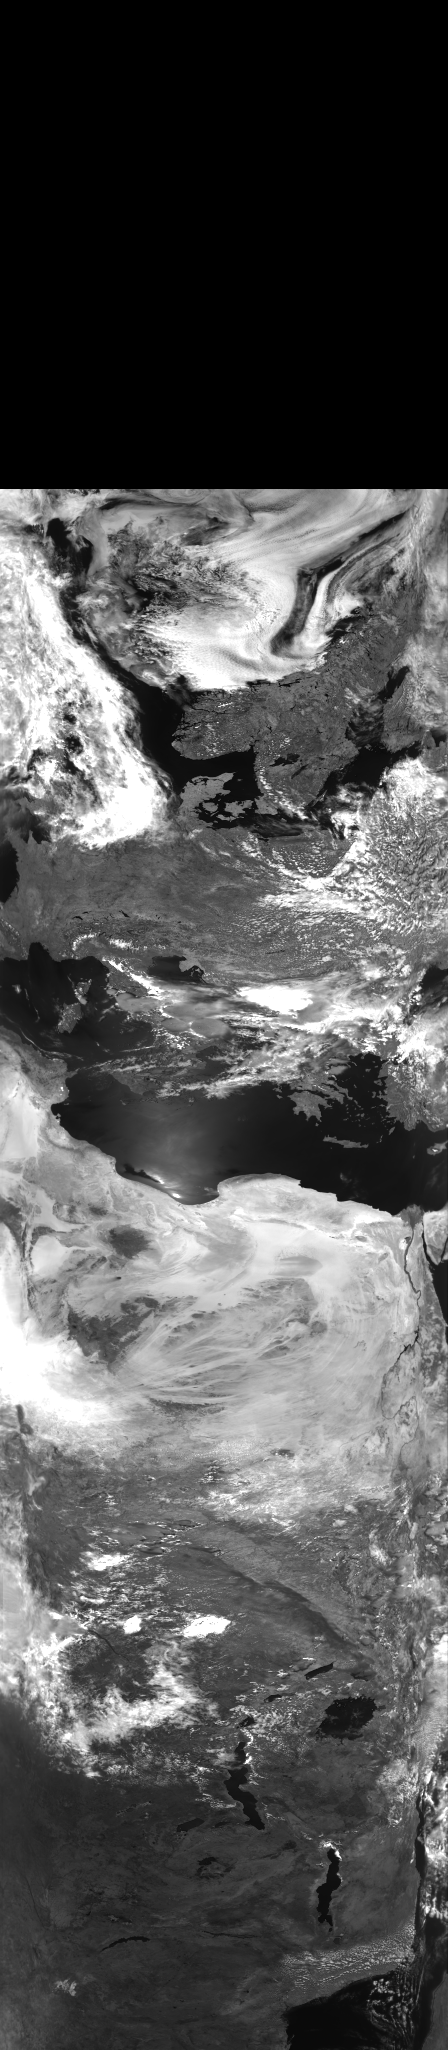
\includegraphics[height=\textheight]{f/s5p_b5_std.png} &
%		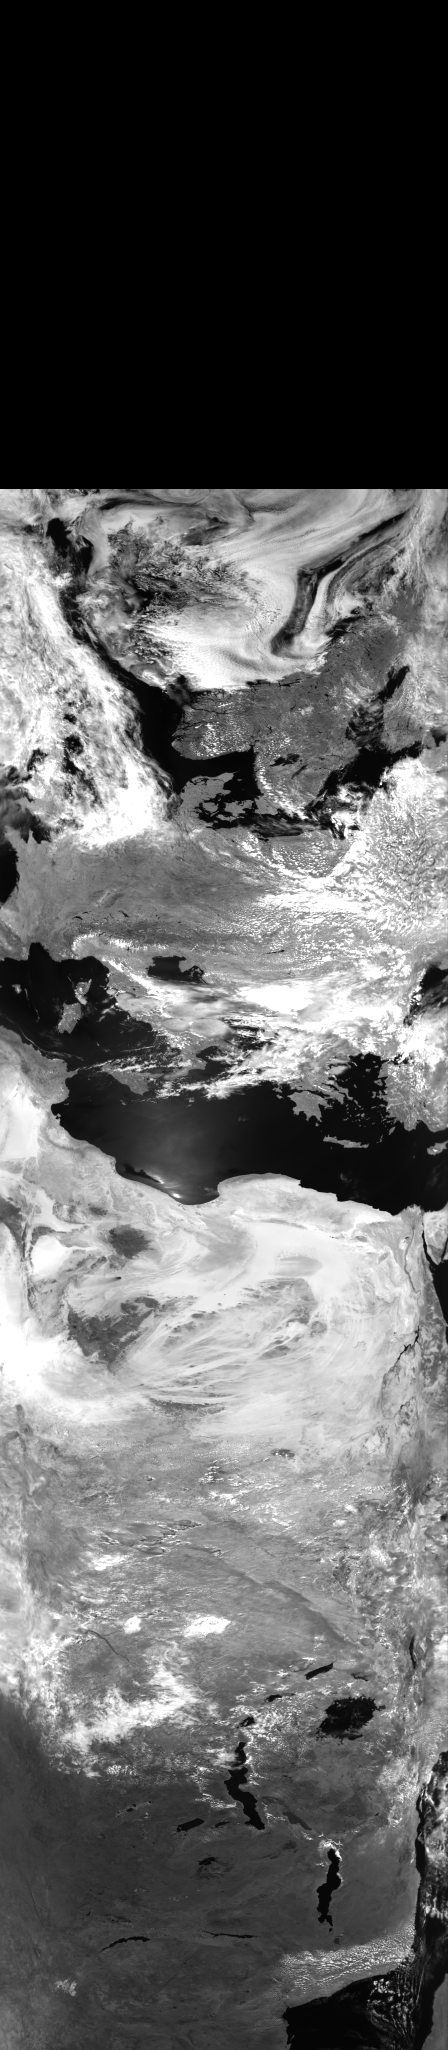
\includegraphics[height=\textheight]{f/s5p_b6_std.png} &
%		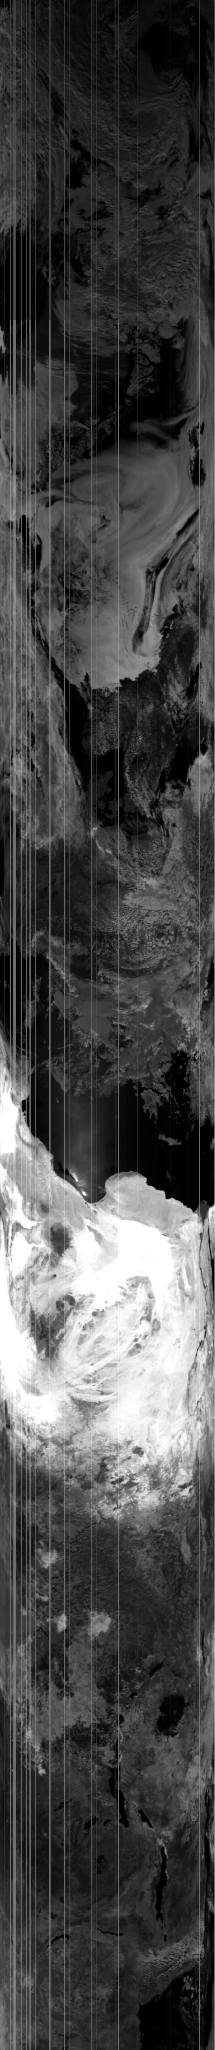
\includegraphics[height=\textheight]{f/s5p_b7_std.png} &
%		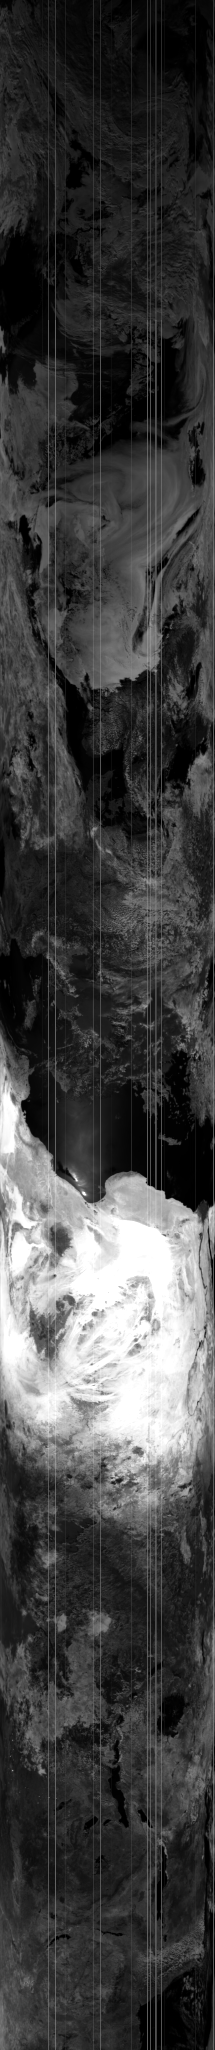
\includegraphics[height=\textheight]{f/s5p_b8_std.png}
%	\end{tabular}
%\end{frame}

% for i in {1..8}; do
%         IIO_TRANS='flip=topdown,y=345,h=2050' plambda ../img/full_L1/o/combi_${i}_{avg,std,iqd}.tif rgb |\
%         qauto -i - f/s5p_b${i}_compo.png
% done
\begin{frame}
	\vspace*{-0.5em}
	\hspace*{-3.1em}
	\tiny
	\renewcommand{\tabcolsep}{0.2pt}
	\begin{tabular}{cccccccc}
		1 UV & 2 UV & 3 UVIS & 4 UVIS & 5 NIR & 6 NIR & 7 SWIR & 8 SWIR \\
		
\includegraphics[height=\textheight]{f/s5p_b1_compo.png} &
		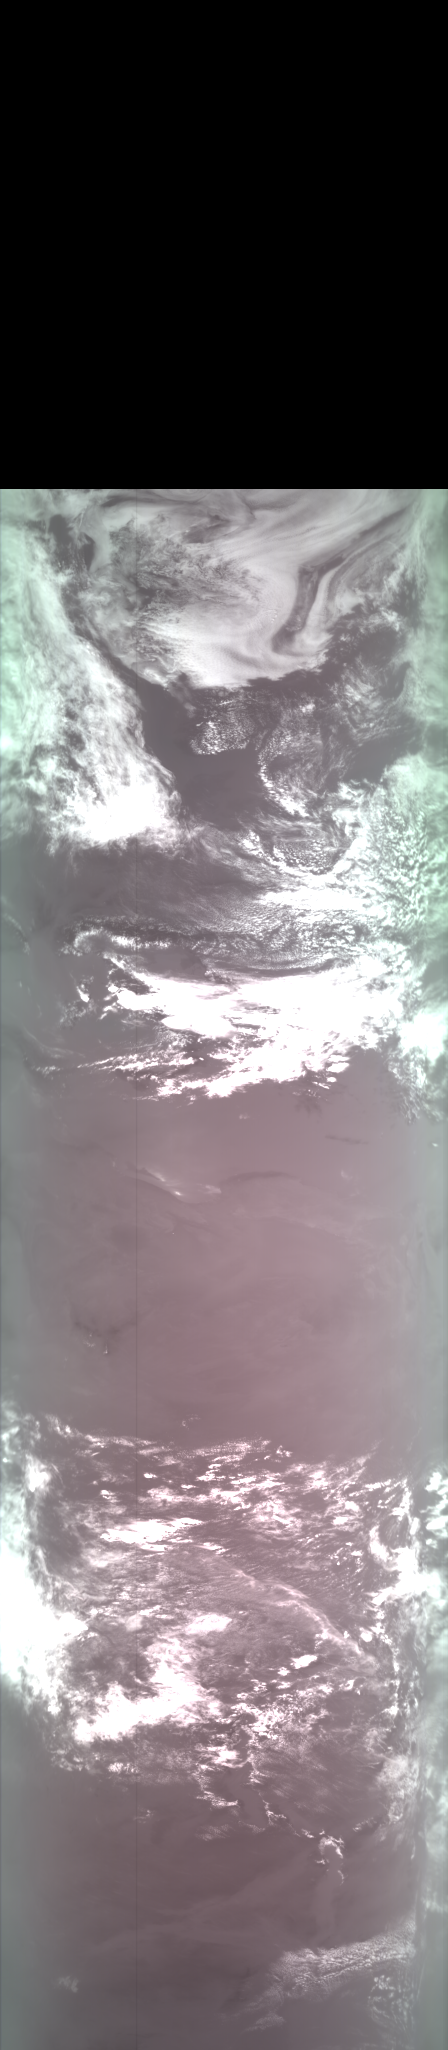
\includegraphics[height=\textheight]{f/s5p_b2_compo.png} &
		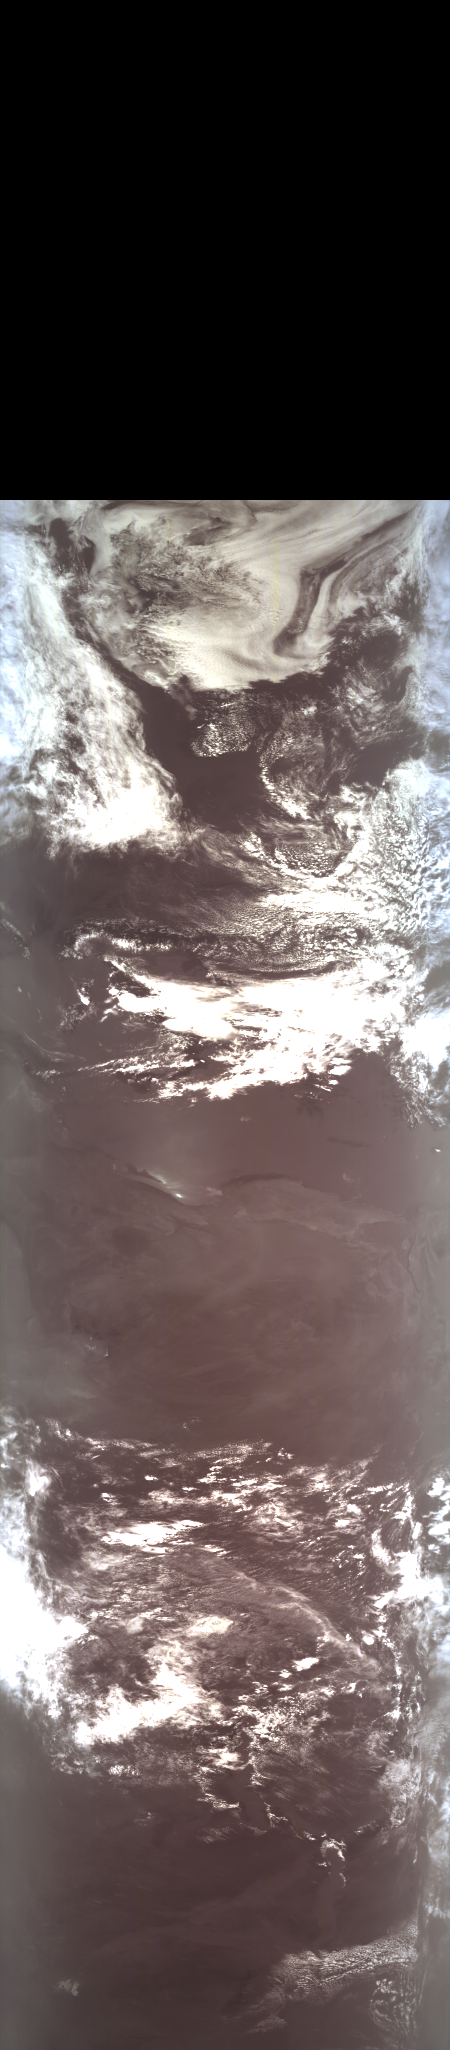
\includegraphics[height=\textheight]{f/s5p_b3_compo.png} &
		
\includegraphics[height=\textheight]{f/s5p_b4_compo.png} &
		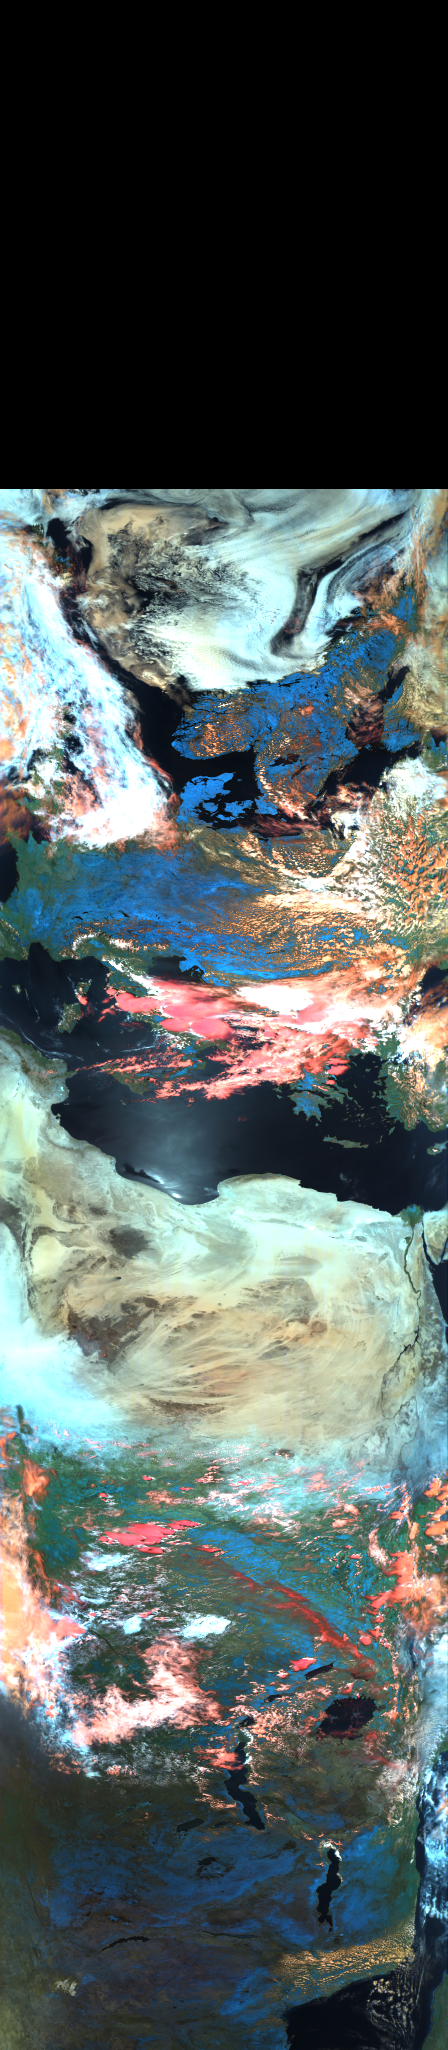
\includegraphics[height=\textheight]{f/s5p_b5_compo.png} &
		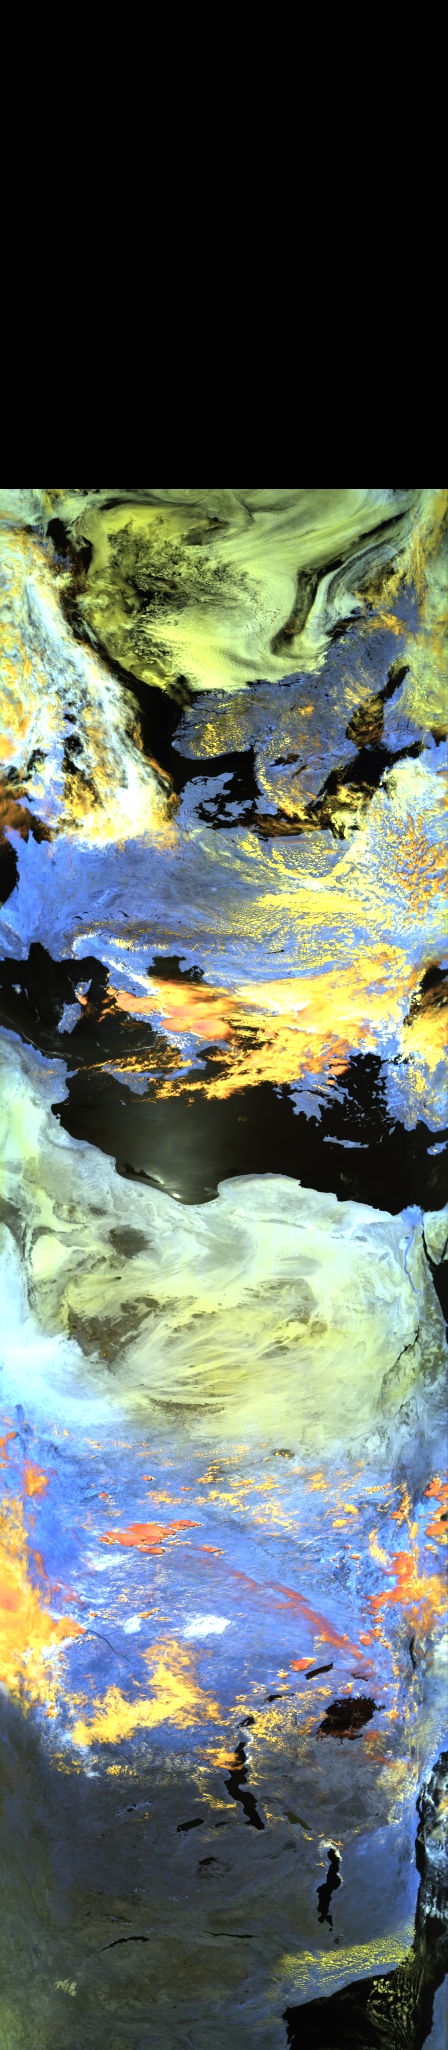
\includegraphics[height=\textheight]{f/s5p_b6_compo.png} &
		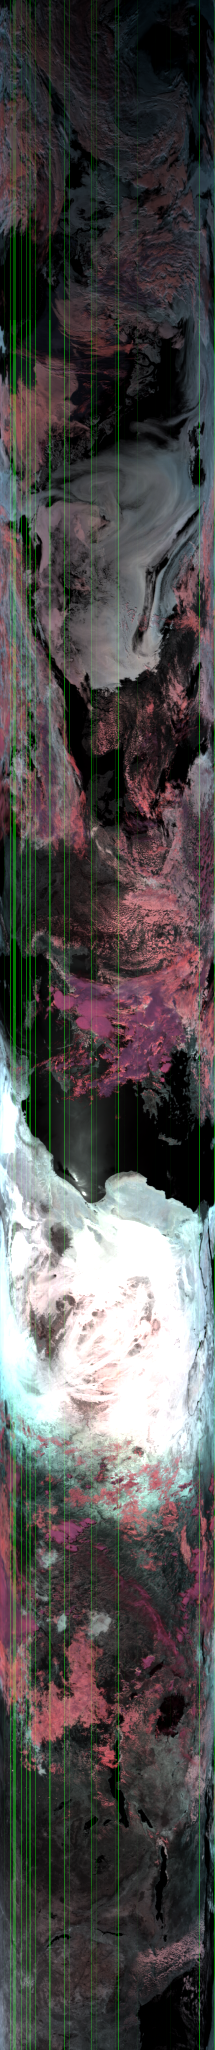
\includegraphics[height=\textheight]{f/s5p_b7_compo.png} &
		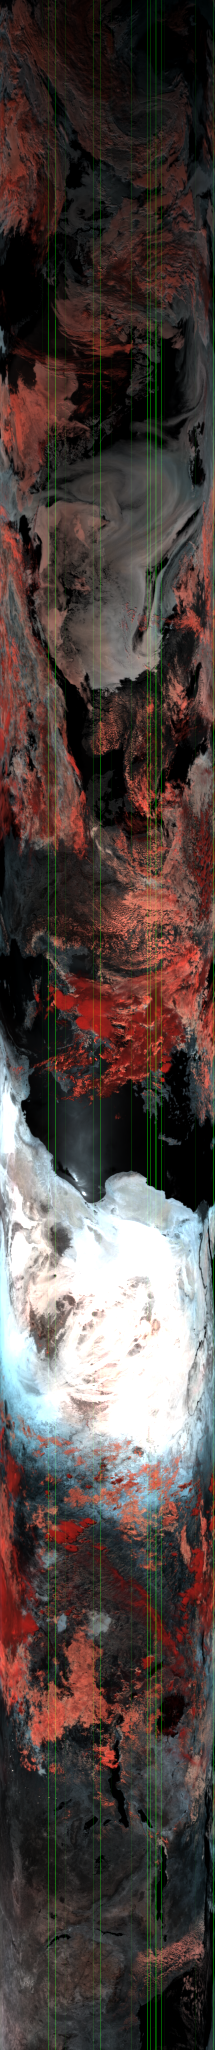
\includegraphics[height=\textheight]{f/s5p_b8_compo.png}
	\end{tabular}
\end{frame}


%for i in 10 292 303 310 335; do qauto -p 2 TRANS[h=1400]:../img/full_L1 /o/s/r6_$i.tif f/r6_$i.png ; done
\begin{frame}
BAND 6, SOME INDIVIDUAL ``WAVELENGTHS''\\
=======================================

\vfill
\renewcommand{\tabcolsep}{1pt}
\begin{tabular}{ccccc}
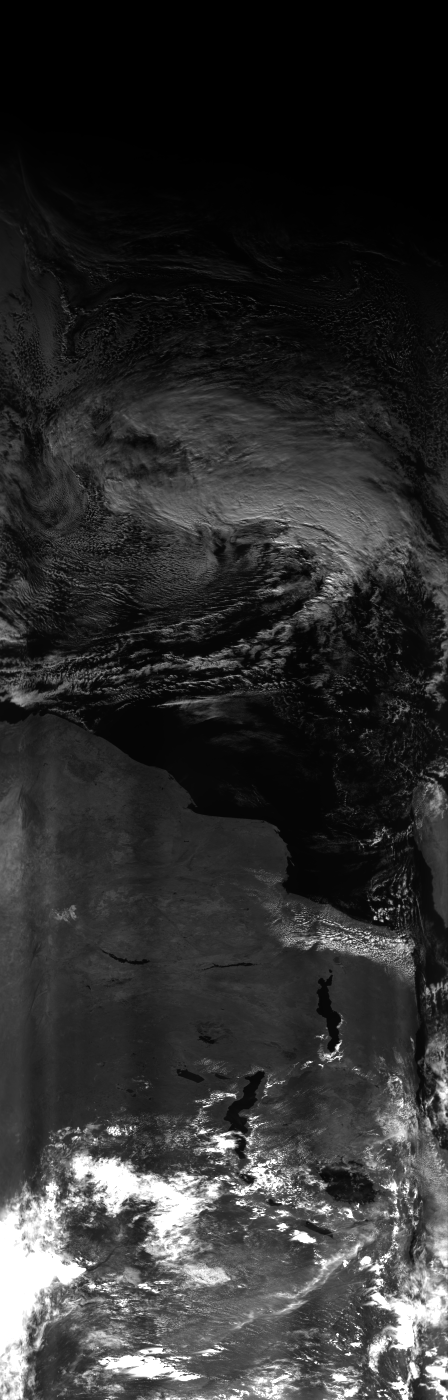
\includegraphics[width=.2\linewidth]{f/r6_10.png} &
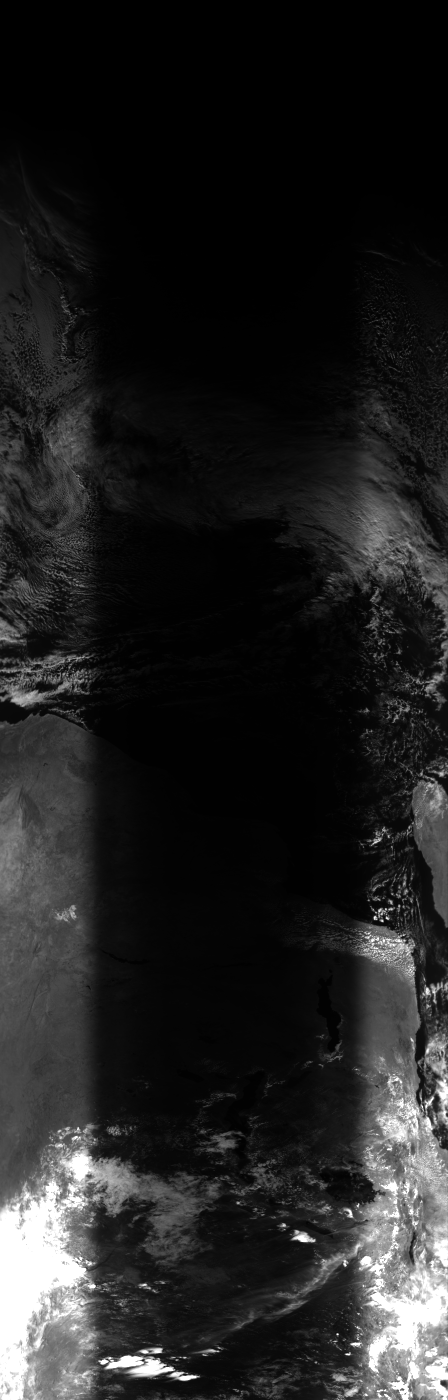
\includegraphics[width=.2\linewidth]{f/r6_292.png} &
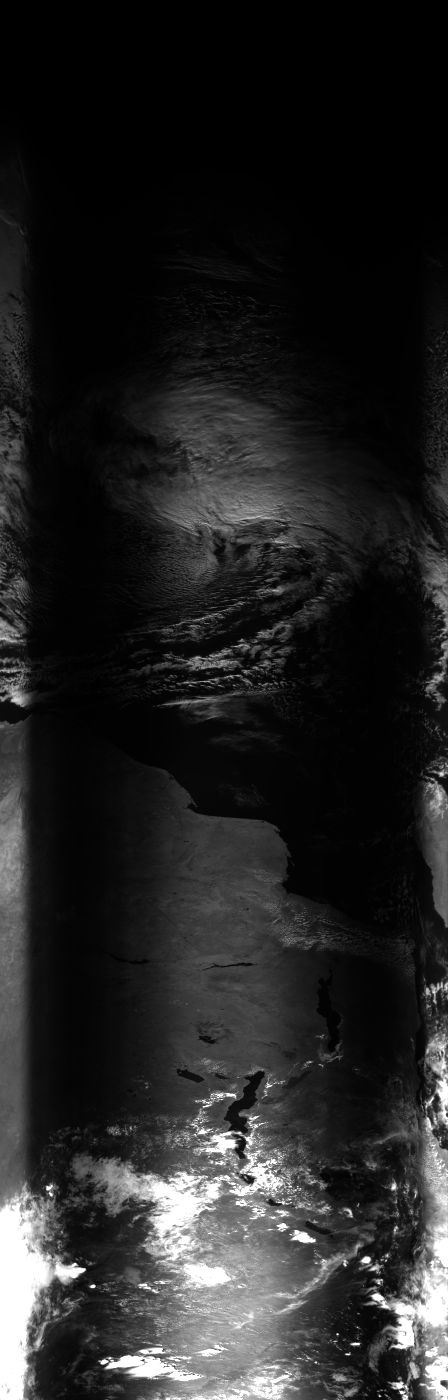
\includegraphics[width=.2\linewidth]{f/r6_303.png} &
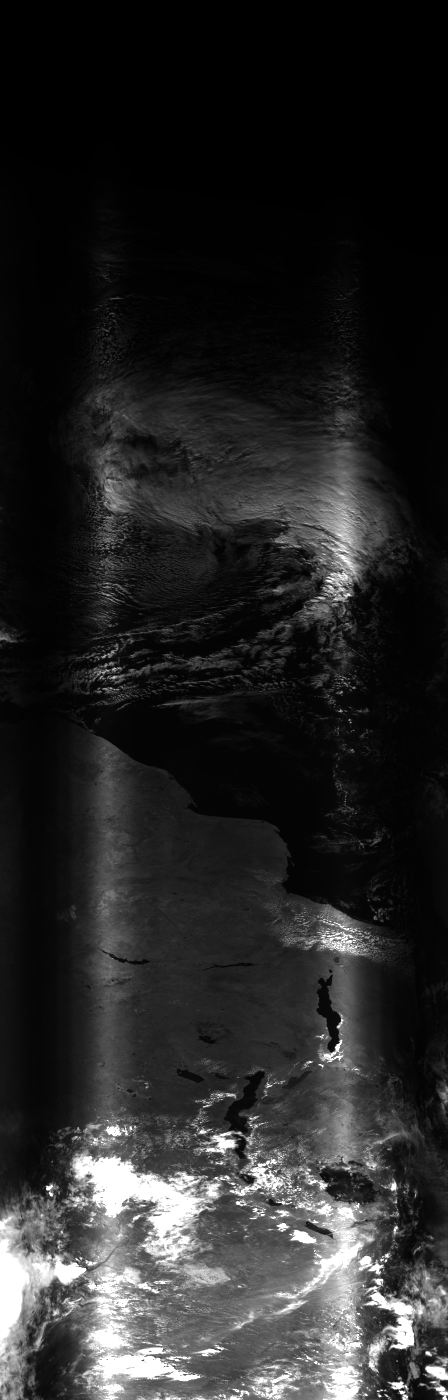
\includegraphics[width=.2\linewidth]{f/r6_310.png} &
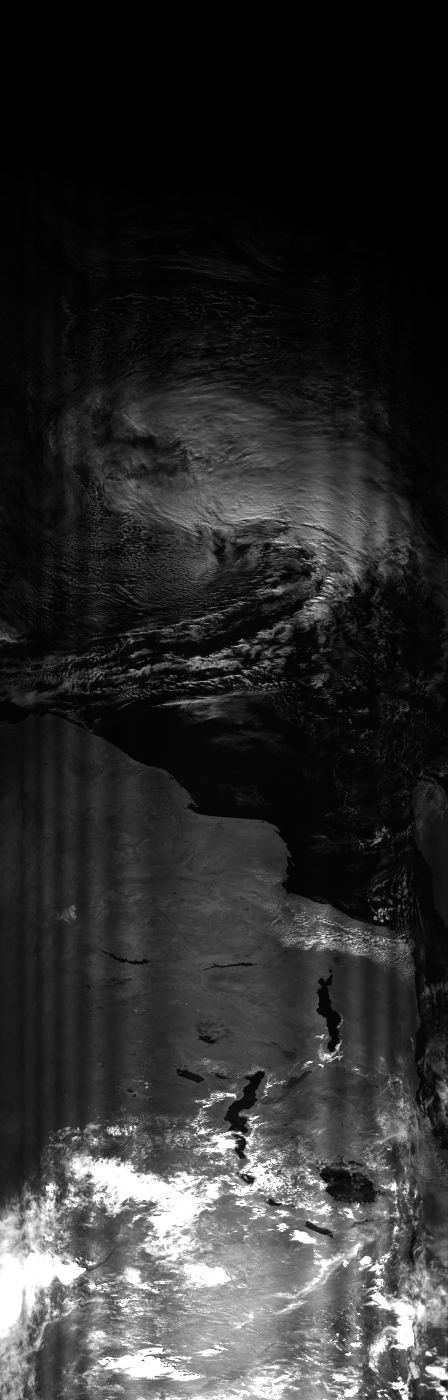
\includegraphics[width=.2\linewidth]{f/r6_335.png} \\
10 & 292 & 303 & 310 & 335
\end{tabular}
\end{frame}



\begin{frame}
BAND 6, CUT ALONG EACH DIMENSION\\
================================

\vfill
\renewcommand{\tabcolsep}{2pt}
\begin{tabular}{ccc}
	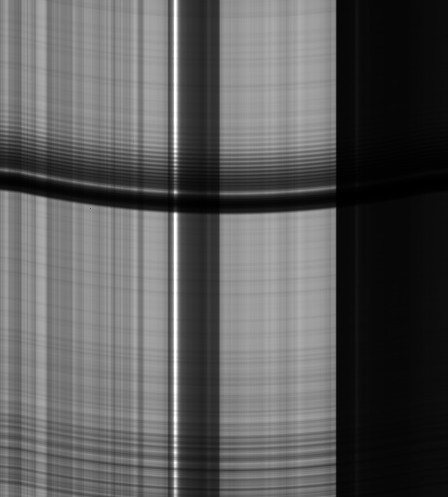
\includegraphics[width=.3\linewidth]{f/kk6_1706.png} &
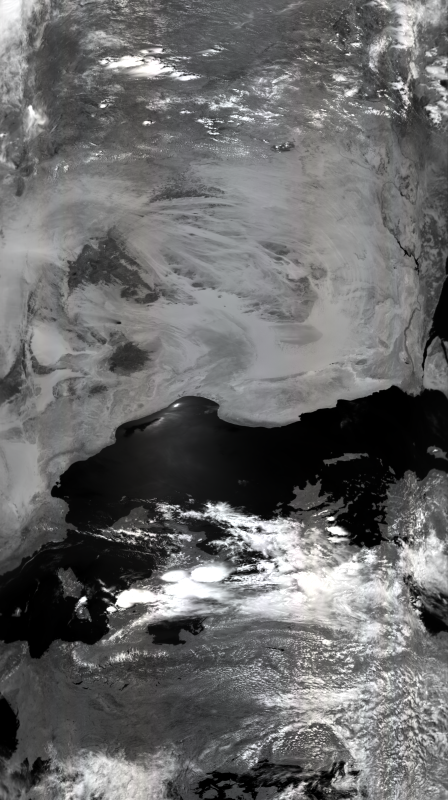
\includegraphics[height=.7\textheight]{f/rgb6_277.png} &

\includegraphics[height=.7\textheight]{f/Tkk6_176.png} \\
y=1706 & z=277 & x=176
\end{tabular}
\end{frame}



%\begin{frame}
%BAND 6, AVERAGE ALONG EACH DIMENSION\\
%====================================
%\end{frame}

\begin{frame}
SPECTROMETER\\
============

\begin{tabular}{ll}
	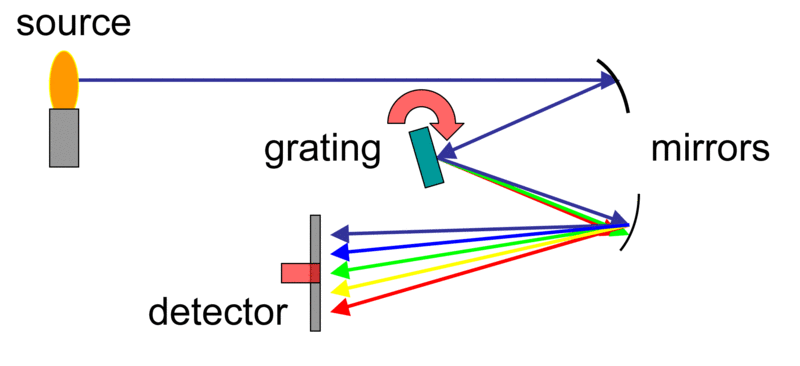
\includegraphics[width=.35\linewidth]{f/spectrometer_wiki.png} &
	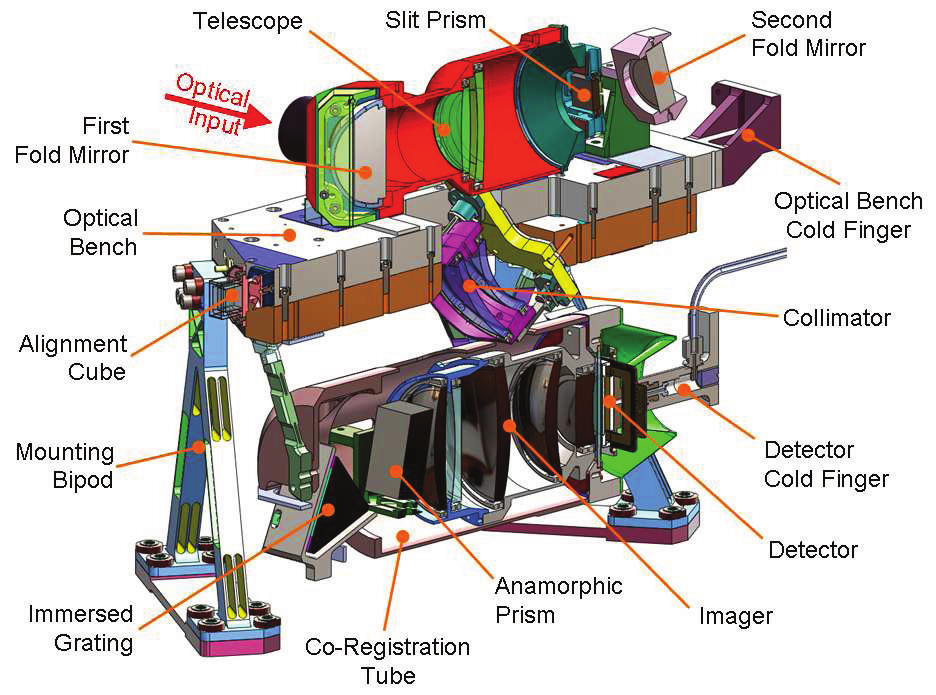
\includegraphics[width=.65\linewidth]{f/spectrometer_esa.png} \\
	\footnotesize wikipedia's spectrometer &
	\footnotesize TROPOMI's SWIR spectrometer
\end{tabular}
\end{frame}

\begin{frame}
NOMINAL WAVELENGTH ALONG ALL BANDS\\
==================================

\vfill

\includegraphics[width=\textwidth]{f/allfreqs.png}\\
\hspace{2em} UV
\hspace{5em} UVIS
\hspace{4em} NIR
\hspace{4em} SWIR

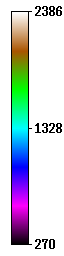
\includegraphics[width=.1\textwidth]{f/pallfreqs.png}
\end{frame}

\begin{frame}
LOCALIZATION AND PROJECTION\\
===========================

The LOCALIZATION function (provided) gives for each sample
at (x,y,z) its (longitude,latitude,wavelength).

Its inverse is the PROJECTION function that allows to get the sample at a given
(longitude,latitude,wavelength).

\vfill

\includegraphics[width=.8\linewidth]{f/splat5_cnt.png}

\end{frame}


\begin{frame}
PROJECTING THE BANDS ONTO THE GROUND\\
====================================

Pixel density at the ground:

\only<1>{
\includegraphics[width=\linewidth]{f/splat1_cnt.png}1}
\only<2>{
\includegraphics[width=\linewidth]{f/splat2_cnt.png}2}
\only<3>{
\includegraphics[width=\linewidth]{f/splat3_cnt.png}3}
\only<4>{\includegraphics[width=\linewidth]{f/splat4_cnt.png}4}
\only<5>{\includegraphics[width=\linewidth]{f/splat5_cnt.png}5}
\only<6>{\includegraphics[width=\linewidth]{f/splat6_cnt.png}6}
\only<7>{\includegraphics[width=\linewidth]{f/splat7_cnt.png}7}
\only<8>{\includegraphics[width=\linewidth]{f/splat8_cnt.png}8}
\end{frame}


\begin{frame}
PROJECTING THE BANDS ONTO THE GROUND\\
====================================

Average band radiance at the ground:

\only<1>{\includegraphics[width=\linewidth]{f/splat1_avg.png}1}
\only<2>{\includegraphics[width=\linewidth]{f/splat2_avg.png}2}
\only<3>{\includegraphics[width=\linewidth]{f/splat3_avg.png}3}
\only<4>{\includegraphics[width=\linewidth]{f/splat4_avg.png}4}
\only<5>{\includegraphics[width=\linewidth]{f/splat5_avg.png}5}
\only<6>{\includegraphics[width=\linewidth]{f/splat6_avg.png}6}
\only<7>{\includegraphics[width=\linewidth]{f/splat7_avg.png}7}
\only<8>{\includegraphics[width=\linewidth]{f/splat8_avg.png}8}
\end{frame}

\begin{frame}
%PROJECTING THE BANDS ONTO THE GROUND\\
%====================================
%
%Average band radiance at the ground:
%
	\only<1>{\includegraphics[width=.85\linewidth]{f/iazplat1.png}1}
	\only<2>{\includegraphics[width=.85\linewidth]{f/iazplat2.png}2}
	\only<3>{\includegraphics[width=.85\linewidth]{f/iazplat3.png}3}
	\only<4>{\includegraphics[width=.85\linewidth]{f/iazplat4.png}4}
	\only<5>{\includegraphics[width=.85\linewidth]{f/iazplat5.png}5}
	\only<6>{\includegraphics[width=.85\linewidth]{f/iazplat6.png}6}
	\only<7>{\includegraphics[width=.85\linewidth]{f/iazplat7.png}7}
	\only<8>{\includegraphics[width=.85\linewidth]{f/iazplat8.png}8}
\end{frame}


\begin{frame}
	\vfill
	2. Extraction of a methane signal from L1 data
	\vfill
\end{frame}


\begin{frame}
EXTRACTION OF A METHANE SIGNAL FROM THE FULL SPECTRUM\\
=====================================================

{\bf Context.}\\
The L1 -> L2/CH4 algorithm is physically-based and extremely complicated

{\bf Idea.}\\
Perform a simple computation that gives similar results

{\bf Recipe.}\\
Compute ratios of particular wavelengths.\\
\pause \color{red}\bf  Which wavelengths?


\end{frame}

\begin{frame}\small
EXTRACTION OF A WAVELENGTH\\
==========================

It is essential to de-quantize the wavelength interpolation
when removing the "smile".

\only<1>{\includegraphics[width=\linewidth]{f/freq_nn.png}}
\only<2>{\includegraphics[width=\linewidth]{f/freq_lin.png}}
%* band 6 cut at a wavelength index
%
%* band 6 interpolated along the smile (nearest-neighbor)
%
%* band 6 interpolated along the smile (linear interpolation)

\end{frame}

\begin{frame}
CLOSEUP OF THE SPECTRUM\\
=======================

\includegraphics[width=\linewidth]{f/whole2_c19.png}
\end{frame}

\begin{frame}
	\includegraphics[width=\linewidth]{f/whole_c19.png}
	\includegraphics[width=\linewidth]{f/whole_c20.png}
	\includegraphics[width=\linewidth]{f/whole_k19.png}
	\includegraphics[width=\linewidth]{f/whole_k20.png}
\end{frame}




%SCRIPT cat <<END | gnuplot > f/curv1920_1.png
%SCRIPT set term pngcairo crop size 900,600
%SCRIPT plot "dat/curv19_1" title "Constantine, 2019, B1" w lines, \
%SCRIPT      "dat/curv20_1" title "Constantine, 2020, B1" w lines
%SCRIPT END
%SCRIPT cat <<END | gnuplot > f/curv1920_2.png
%SCRIPT set term pngcairo crop size 900,600
%SCRIPT plot "dat/curv19_2" title "Constantine, 2019, B2" w lines, \
%SCRIPT      "dat/curv20_2" title "Constantine, 2020, B2" w lines
%SCRIPT END
%SCRIPT cat <<END | gnuplot > f/curv1920_3.png
%SCRIPT set term pngcairo crop size 900,600
%SCRIPT plot "dat/curv19_3" title "Constantine, 2019, B3" w lines, \
%SCRIPT      "dat/curv20_3" title "Constantine, 2020, B3" w lines
%SCRIPT END
%SCRIPT cat <<END | gnuplot > f/curv1920_4.png
%SCRIPT set term pngcairo crop size 900,600
%SCRIPT plot "dat/curv19_4" title "Constantine, 2019, B4" w lines, \
%SCRIPT      "dat/curv20_4" title "Constantine, 2020, B4" w lines
%SCRIPT END
%SCRIPT cat <<END | gnuplot > f/curv1920_5.png
%SCRIPT set term pngcairo crop size 900,600
%SCRIPT plot "dat/curv19_5" title "Constantine, 2019, B5" w lines, \
%SCRIPT      "dat/curv20_5" title "Constantine, 2020, B5" w lines
%SCRIPT END
%SCRIPT cat <<END | gnuplot > f/curv1920_6.png
%SCRIPT set term pngcairo crop size 900,600
%SCRIPT plot "dat/curv19_6" title "Constantine, 2019, B6" w lines, \
%SCRIPT      "dat/curv20_6" title "Constantine, 2020, B6" w lines
%SCRIPT END
%SCRIPT cat <<END | gnuplot > f/curv1920_7.png
%SCRIPT set term pngcairo crop size 900,600
%SCRIPT plot "dat/curv19_7" title "Constantine, 2019, B7" w lines, \
%SCRIPT      "dat/curv20_7" title "Constantine, 2020, B7" w lines
%SCRIPT END
%SCRIPT cat <<END | gnuplot > f/curv1920_8.png
%SCRIPT set term pngcairo crop size 900,600
%SCRIPT plot "dat/curv19_8" title "Constantine, 2019, B8" w lines, \
%SCRIPT      "dat/curv20_8" title "Constantine, 2020, B8" w lines
%SCRIPT END

%SCRIPT cat <<END | gnuplot > f/curv1920_12.png
%SCRIPT set term pngcairo crop size 900,600
%SCRIPT plot "< cat dat/curv19_[1,2]" title "Constantine, 2019, UV" w lines, \
%SCRIPT      "< cat dat/curv20_[1,2]" title "Constantine, 2020, UV" w lines
%SCRIPT END
%SCRIPT cat <<END | gnuplot > f/curv1920_34.png
%SCRIPT set term pngcairo crop size 900,600
%SCRIPT plot "< cat dat/curv19_[3,4]" title "Constantine, 2019, UVIS" w lines, \
%SCRIPT      "< cat dat/curv20_[3,4]" title "Constantine, 2020, UVIS" w lines
%SCRIPT END
%SCRIPT cat <<END | gnuplot > f/curv1920_56.png
%SCRIPT set term pngcairo crop size 900,600
%SCRIPT plot "< cat dat/curv19_[5,6]" title "Constantine, 2019, NIR" w lines, \
%SCRIPT      "< cat dat/curv20_[5,6]" title "Constantine, 2020, NIR" w lines
%SCRIPT END
%SCRIPT cat <<END | gnuplot > f/curv1920_78.png
%SCRIPT set term pngcairo crop size 900,600
%SCRIPT plot "< cat dat/curv19_[7,8]" title "Constantine, 2019, SWIR" w lines, \
%SCRIPT      "< cat dat/curv20_[7,8]" title "Constantine, 2020, SWIR" w lines
%SCRIPT END

\begin{frame}
CLOSEUP OF THE SPECTRUM (constantine, two dates)\\
================================================
\vfill

\only<1>{\includegraphics[width=\linewidth]{f/curv1920_12.png}}
\only<2>{\includegraphics[width=\linewidth]{f/curv1920_34.png}}
\only<3>{\includegraphics[width=\linewidth]{f/curv1920_56.png}}
\only<4>{\includegraphics[width=\linewidth]{f/curv1920_78.png}}
\end{frame}




%SCRIPT cat <<END | gnuplot > f/ckurv19_1.png
%SCRIPT set term pngcairo crop size 900,600
%SCRIPT plot "dat/curv19_1" title "Constantine, 2019, B1" w lines, \
%SCRIPT      "dat/kurv19_1" title "Ouargla, 2019, B1" w lines
%SCRIPT END
%SCRIPT cat <<END | gnuplot > f/ckurv19_2.png
%SCRIPT set term pngcairo crop size 900,600
%SCRIPT plot "dat/curv19_2" title "Constantine, 2019, B2" w lines, \
%SCRIPT      "dat/kurv19_2" title "Ouargla, 2019, B2" w lines
%SCRIPT END
%SCRIPT cat <<END | gnuplot > f/ckurv19_3.png
%SCRIPT set term pngcairo crop size 900,600
%SCRIPT plot "dat/curv19_3" title "Constantine, 2019, B3" w lines, \
%SCRIPT      "dat/kurv19_3" title "Ouargla, 2019, B3" w lines
%SCRIPT END
%SCRIPT cat <<END | gnuplot > f/ckurv19_4.png
%SCRIPT set term pngcairo crop size 900,600
%SCRIPT plot "dat/curv19_4" title "Constantine, 2019, B4" w lines, \
%SCRIPT      "dat/kurv19_4" title "Ouargla, 2019, B4" w lines
%SCRIPT END
%SCRIPT cat <<END | gnuplot > f/ckurv19_5.png
%SCRIPT set term pngcairo crop size 900,600
%SCRIPT plot "dat/curv19_5" title "Constantine, 2019, B5" w lines, \
%SCRIPT      "dat/kurv19_5" title "Ouargla, 2019, B5" w lines
%SCRIPT END
%SCRIPT cat <<END | gnuplot > f/ckurv19_6.png
%SCRIPT set term pngcairo crop size 900,600
%SCRIPT plot "dat/curv19_6" title "Constantine, 2019, B6" w lines, \
%SCRIPT      "dat/kurv19_6" title "Ouargla, 2019, B6" w lines
%SCRIPT END
%SCRIPT cat <<END | gnuplot > f/ckurv19_7.png
%SCRIPT set term pngcairo crop size 900,600
%SCRIPT plot "dat/curv19_7" title "Constantine, 2019, B7" w lines, \
%SCRIPT      "dat/kurv19_7" title "Ouargla, 2019, B7" w lines
%SCRIPT END
%SCRIPT cat <<END | gnuplot > f/ckurv19_8.png
%SCRIPT set term pngcairo crop size 900,600
%SCRIPT plot "dat/curv19_8" title "Constantine, 2019, B8" w lines, \
%SCRIPT      "dat/kurv19_8" title "Ouargla, 2019, B8" w lines
%SCRIPT END

\begin{frame}
CLOSEUP OF THE SPECTRUM (constantine/ouargla, 2019)\\
===================================================
\vfill

\only<1>{\includegraphics[width=\linewidth]{f/ckurv19_1.png}}
\only<2>{\includegraphics[width=\linewidth]{f/ckurv19_2.png}}
\only<3>{\includegraphics[width=\linewidth]{f/ckurv19_3.png}}
\only<4>{\includegraphics[width=\linewidth]{f/ckurv19_4.png}}
\only<5>{\includegraphics[width=\linewidth]{f/ckurv19_5.png}}
\only<6>{\includegraphics[width=\linewidth]{f/ckurv19_6.png}}
\only<7>{\includegraphics[width=\linewidth]{f/ckurv19_7.png}}
\only<8>{\includegraphics[width=\linewidth]{f/ckurv19_8.png}}
\end{frame}

%SCRIPT cat <<END | gnuplot > f/kurv1920_1.png
%SCRIPT set term pngcairo crop size 900,600
%SCRIPT plot "dat/kurv19_1" title "Ouargla, 2019, B1" w lines, \
%SCRIPT      "dat/kurv20_1" title "Ouargla, 2020, B1" w lines
%SCRIPT END
%SCRIPT cat <<END | gnuplot > f/kurv1920_2.png
%SCRIPT set term pngcairo crop size 900,600
%SCRIPT plot "dat/kurv19_2" title "Ouargla, 2019, B2" w lines, \
%SCRIPT      "dat/kurv20_2" title "Ouargla, 2020, B2" w lines
%SCRIPT END
%SCRIPT cat <<END | gnuplot > f/kurv1920_3.png
%SCRIPT set term pngcairo crop size 900,600
%SCRIPT plot "dat/kurv19_3" title "Ouargla, 2019, B3" w lines, \
%SCRIPT      "dat/kurv20_3" title "Ouargla, 2020, B3" w lines
%SCRIPT END
%SCRIPT cat <<END | gnuplot > f/kurv1920_4.png
%SCRIPT set term pngcairo crop size 900,600
%SCRIPT plot "dat/kurv19_4" title "Ouargla, 2019, B4" w lines, \
%SCRIPT      "dat/kurv20_4" title "Ouargla, 2020, B4" w lines
%SCRIPT END
%SCRIPT cat <<END | gnuplot > f/kurv1920_5.png
%SCRIPT set term pngcairo crop size 900,600
%SCRIPT plot "dat/kurv19_5" title "Ouargla, 2019, B5" w lines, \
%SCRIPT      "dat/kurv20_5" title "Ouargla, 2020, B5" w lines
%SCRIPT END
%SCRIPT cat <<END | gnuplot > f/kurv1920_6.png
%SCRIPT set term pngcairo crop size 900,600
%SCRIPT plot "dat/kurv19_6" title "Ouargla, 2019, B6" w lines, \
%SCRIPT      "dat/kurv20_6" title "Ouargla, 2020, B6" w lines
%SCRIPT END
%SCRIPT cat <<END | gnuplot > f/kurv1920_7.png
%SCRIPT set term pngcairo crop size 900,600
%SCRIPT plot "dat/kurv19_7" title "Ouargla, 2019, B7" w lines, \
%SCRIPT      "dat/kurv20_7" title "Ouargla, 2020, B7" w lines
%SCRIPT END
%SCRIPT cat <<END | gnuplot > f/kurv1920_8.png
%SCRIPT set term pngcairo crop size 900,600
%SCRIPT plot "dat/kurv19_8" title "Ouargla, 2019, B8" w lines, \
%SCRIPT      "dat/kurv20_8" title "Ouargla, 2020, B8" w lines
%SCRIPT END

\begin{frame}
CLOSEUP OF THE SPECTRUM (ouargla, two dates)\\
================================================
\vfill

\only<1>{\includegraphics[width=\linewidth]{f/kurv1920_1.png}}
\only<2>{\includegraphics[width=\linewidth]{f/kurv1920_2.png}}
\only<3>{\includegraphics[width=\linewidth]{f/kurv1920_3.png}}
\only<4>{\includegraphics[width=\linewidth]{f/kurv1920_4.png}}
\only<5>{\includegraphics[width=\linewidth]{f/kurv1920_5.png}}
\only<6>{\includegraphics[width=\linewidth]{f/kurv1920_6.png}}
\only<7>{\includegraphics[width=\linewidth]{f/kurv1920_7.png}}
\only<8>{\includegraphics[width=\linewidth]{f/kurv1920_8.png}}
\only<9>{\includegraphics[width=\linewidth]{f/ckurv19_8.png}}
\end{frame}


\begin{frame}
HEURISTIC METHANE RECIPE\\
========================

1. Slice the images at 4 particular frequencies on band 8
\[
	\omega_1 = 2346.6
	\qquad
	\omega_2 = 2349.5
	\qquad
	\omega_3 = 2350.5
	\qquad
	\omega_4 = 2356.1
\]

2. Build a 3-channel image of ratios
$$u=\left(\omega_2/\omega_3,\ \omega_1/\omega_4,\ \omega_2/\omega_4\right)$$

3. Normalize the contrast to obtain a 8-bit RGB image

\end{frame}

\begin{frame}
HEURISTIC METHANE\\
=================

\begin{tabular}{ll}
	\includegraphics[height=.7\textheight]{f/ccplume20.png} &
	\includegraphics[height=.7\textheight]{f/niceshot.png} \\
	L2 product & Heuristic from L1
\end{tabular}
\end{frame}

\begin{frame}
HEURISTIC METHANE\\
=================

\begin{tabular}{ll}
	\includegraphics[height=.7\textheight]{f/kccplume20.png} &
	\includegraphics[height=.7\textheight]{f/ikniceshot.png} \\
	L2 product & Heuristic from L1
\end{tabular}
\end{frame}



\begin{frame}
COMPARISON L2 L1 (orbit
\only<1>{11536}\only<2>{11522}\only<3>{11550}\only<4>{11564})\\
==============================

\vfill

\begin{tabular}{ll}
\only<1>{\includegraphics[width=.5\textwidth]{f/imeth_11536.png}}%
\only<2>{\includegraphics[width=.5\textwidth]{f/imeth_11522.png}}%
\only<3>{\includegraphics[width=.5\textwidth]{f/imeth_11550.png}}%
\only<4>{\includegraphics[width=.5\textwidth]{f/imeth_11564.png}}%
	&
\only<1>{\includegraphics[width=.5\textwidth]{f/view_11536.png}}%
\only<2>{\includegraphics[width=.5\textwidth]{f/view_11522.png}}%
\only<3>{\includegraphics[width=.5\textwidth]{f/view_11550.png}}%
\only<4>{\includegraphics[width=.5\textwidth]{f/view_11564.png}}%
	\\
	Ouargla L2 & Ouargla L1
\end{tabular}
\end{frame}

\begin{frame}
HUGE PLUME ACROSS THE ARABIAN PENINSULA\\
\includegraphics[width=.8\textwidth]{f/iraqui_plume.png}

\small
{\bf Orbit 08074.}
Notice huge light-blue semitransparent plume.  It is transparent
to visible light.  Most probably not methane (too large!)
\end{frame}



\begin{frame}
ONGOING WORK\\
============

* We understand how to extract data from TROPOMI L1 files

* By matching the L1 and L2-CH4 products, we are trying to learn their 
correspondence using simple models, e.g.

- a classifier of plume/non plume

- the whole mapping (radiance) -> (methane-mixing-ratio)



\end{frame}



\begin{frame}
STATUS\\
======

0. Methane plumes can be ``seen'' as sligthly darker samples on a few
particular frequency ratios.

1. A methane signal can be reliably obtained from L1 data
(without ``holes'', but without units)

2. It may be technically feasible to download only a small part of the L1
products to perform this computation.

3. Technical quests:\\
3.1. remove the ``stripes'' (easy)\\
3.2. remove the ``halos'' (easy)\\
3.3. use LEARNED ratios instead of hand picked (hard)
\end{frame}

\end{document}


% vim:sw=2 ts=2 spell spelllang=en:
